\textbf{Ejemplo 1}\\

Dos ciudades A y B están unidos mediante una vieja carretera y se proyecta la construcción de una nueva carretera que costará   COP  100 millones y que acortará el camino entre éstas dos ciudades. Esto implica una disminución en el consumo del combustible, aceites, desgaste de vehículos y en el valor del peaje. Todas estas disminuciones se estiman que pueden llegar a valer   COP  28 millones al año. Por otra parte, hay varios comerciantes que han montado restaurantes y hoteles a lo largo de la carretera antigua y con la construcción de la nueva carretera el perjuicio que recibirán estos por la disminución del turismo, ascendería a   COP  15 millones al año. Utilizando la Relación B/C determinar la conveniencia del proyecto utilizando:
\\

\textbf{Solución.}\\
%La tabla ira centrada
\begin{center}
	\renewcommand{\arraystretch}{1.5}% Margenes de las celdas
	%Creación de la cuadricula de 3 columnas
\begin{longtable}[H]{|c|c|c|}
		%Creamos una linea horizontal
\hline
		%Definimos el color de la primera fila
\rowcolor[HTML]{FFB183}
	%%%%% INICIO ASIGNACIÓN PERÍODO FOCAL %%%%%%%
  %%%%%%%%%% INICIO TITULO
  %Lo que se hace aquí es mezclar las 3 columnas en una sola
  \multicolumn{3}{|c|}{\cellcolor[HTML]{FFB183}\textbf{1. Asignación período focal}}   \\ \hline
  %%%%%%%%%% FIN TITULO
  %%%%% INICIO DECLARACIÓN DE VARIABLES %%%%%%%
  \multicolumn{3}{|c|}{$pf =0 pav$}   \\ \hline
  %%%%% INICIO DECLARACIÓN FORMULAS
  
%%%%%%%%%%% INICIO TITULO
\rowcolor[HTML]{FFB183}
\multicolumn{3}{|c|}{\cellcolor[HTML]{FFB183}\textbf{2. Declaración de variables}}    \\ \hline
%%%%%%%%%%% FIN TITULO
%%%%%%%%%%% INICIO MATEMÁTICAS

$R =   COP  100  \text{ millones Para una serie infinita}$                                     & \multicolumn{2}{c|}{$ i_1 = 30\% pav $} \\
$ValorDisminucion =   COP  28 millones $	& \multicolumn{2}{c|}{$ i_2 = 12\% pav $} \\
$ Inversion_1 =   COP  15 millones $	&	\multicolumn{2}{c|}{ $ VPN =  COP  ? $ } \\ 
$ $	&	\multicolumn{2}{c|}{ $ VP =  COP  ? $ } \\ 

\hline
%%%%%%%%%% FIN MATEMÁTICAS
		%%%%% INICIO FLUJO DE CAJA
\rowcolor[HTML]{FFB183}
\multicolumn{3}{|c|}{\cellcolor[HTML]{FFB183}\textbf{3. Diagrama de flujo de caja}} \\ \hline
		%Mezclamos 3 columnas y pondremos el dibujo
		%%%%%%%%%%%%% INSERCIÓN DE LA IMAGEN
		%Deberán descargar las imágenes respectivas del drive y pegarlas en la carpeta
		%n_capitulo/img/ejemplos/1/capitulo1ejemplo1.pdf  (el /1/ es el numero del ejemplo)
\multicolumn{3}{|c|}{ 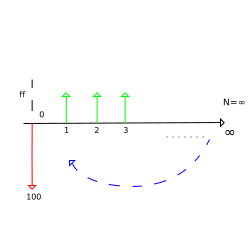
\includegraphics[height=6cm]{E12_2.pdf}}   
   \\ \hline
		%%%%%%%%%%%%% FIN INSERCIÓN DE IMAGEN
		%%%%%FIN FLUJO DE CAJA
		
		
		
		%%%%% INICIO DECLARACIÓN FORMULAS
		%%%%%%%%%%% INICIO TITULO
\rowcolor[HTML]{FFB183}
\multicolumn{3}{|c|}{\cellcolor[HTML]{FFB183}\textbf{4. Declaración de fórmulas}}    \\ \hline
		%%%%%%%%%%% FIN TITULO
		%%%%%%%%%%% INICIO MATEMÁTICAS
\multicolumn{3}{|c|} {$VPN = \Sigma(Costos) - \Sigma(Inversiones) $\hspace{15pt}\textit{Valor Presente Neto}}   \\ 
\multicolumn{3}{|c|} {$VP = \frac{R}{i}$\hspace{15pt}\textit{ Valor Presente para una Serie Perpetua Vencida}}   \\ 
\multicolumn{3}{|c|} {$B/C = \frac{VPN}{VPC}$\hspace{15pt}\textit{ Relación Beneficio/Costo}}   \\ 
\hline	
	
		%%%%%%%%%% FIN MATEMÁTICAS
		%%%%%% INICIO DESARROLLO MATEMÁTICO
\rowcolor[HTML]{FFB183}
		%%%%%%%%%%INICIO TITULO
\multicolumn{3}{|c|}{\cellcolor[HTML]{FFB183}\textbf{5. Desarrollo matemático}}       \\ \hline
		%%%%%%%%%% FIN TITULO
		%%%%%%%%%% INICIO MATEMÁTICAS
		\multicolumn{3}{|c|}{$\quad \quad \quad \quad \quad \quad VPN =   COP   28 millones -   COP   15 millones =   COP  13 millones \quad \quad \quad \quad \quad \quad $}  
		\\
		
		\multicolumn{3}{|c|}{$ R = (  COP   100 millones)(0.3) =   COP  30 millones$}  
		\\
	
		\multicolumn{3}{|c|}{$ B/C = \frac{13}{30} = 0.43 < 1 $}
		\\ 
		\multicolumn{3}{|c|}{$ VPN = -100 + 13/0.3 = -  COP  50.07 millones $}
		\\ 
		\multicolumn{3}{|c|}{$ X =   COP  100 millones(0.12) =   COP  12 \text{millones el año} $}
		\\ 
		\multicolumn{3}{|c|}{$ \phi = VP(i) \hspace{15pt} \textit{Valor Presente para una serie infinita anual } $}
		\\ 
		\multicolumn{3}{|c|}{$ \phi =   COP  100(0.3) =   COP  30  millones $}
		\\ 
		\multicolumn{3}{|c|}{$ \text{entonces el índice será}  $}
		\\ 
		\multicolumn{3}{|c|}{$ B/C = \frac{28-15}{12} = 1.0833 > 1 $}
		\\ 
		\multicolumn{3}{|c|}{$ B/C = \frac{13}{30} = 0.43 < 1 $}
		\\ 
		\hline
				
		%%%%%%%%%% FIN MATEMÁTICAS
		%%%%%% FIN DESARROLLO MATEMÁTICO
		%%%%%% INICIO RESPUESTA
\rowcolor[HTML]{FFB183}
		%%%%%%%%%%INICIO TITULO
\multicolumn{3}{|c|}{\cellcolor[HTML]{FFB183}\textbf{6. Respuesta}}   \\ \hline
		%%%%%%%%%% FIN TITULO
		%%%%%%%%%% INICIO RESPUESTA MATEMÁTICA
		
\multicolumn{3}{|c|}{ $ VPN = -100 + 13/0.3 = -  COP  56.67 millones $ }  \\ 
\multicolumn{3}{|c|}{ $ \text{Esto da un VPN negativo } $ }  \\ 
\multicolumn{3}{|c|}{ $ B/C=\frac{28-15}{12} = 1.0833 > 1 $ }  \\ 
\multicolumn{3}{|c|}{ $ \textbf{Por tal razón el proyecto no es aconsejable} $ }  \\ 
\hline
		
		
		%%%%%%%%%% FIN MATEMÁTICAS
		%%%%%% FIN RESPUESTA
	\end{longtable}
	%Se crean dos lineas en blanco para que no quede el siguiente texto tan pegado
	%\newline \newline %USARLO SI CREES QUE ES NECESARIO
\end{center}
%%%%%%%%%%%%%%%%%%%%%%%%%%FIN EJERCICIO 1 %%%%%%%%%%%%%%%%%%%%%%%%%%%
